\chapter{小型低性能計算機を用いたマルチディスプレイシステムの構築}

本章では,小型低性能計算機,特にSBCを利用した低コストなマルチディスプレイシステム構築手法の必要性と,その実現に向けて行われた先行研究について説明する.
まず2.1節では,従来利用されてきたマルチディスプレイシステムの構築手法とそのコストについて述べる.
続く2.2節では,先行研究でも使用されており,本研究でも取り扱うシングルボードコンピュータ (SBC) について説明し,2.3節では先行研究である,SBCを用いて構築されたマルチディスプレイシステムについて説明する.
さらに2.4節で,先行研究で提案されたSBCを用いたマルチディスプレイシステムについての問題点と,その問題点を解決することを目的として行われた関連研究を紹介する.
最後に2.5節では関連研究において将来的な課題とされていた部分の改善策と,それを実現するための技術的な課題点について述べる.

\section{従来のマルチディスプレイ構築手法}
これまでMDの構築には数多くの手法が提案されており,それらは大きく分けると2種類の手法に分類することができる\cite{pccluster,6693038}.
1つは専用のハードウェアを用いてマルチディスプレイを構築する手法であり,もう1つは専用のミドルウェアを用いてマルチディスプレイを構築する手法である.
本節では,この2種類の構築手法を簡単に解説してそれぞれの構成例を示し,構築に要する金銭的コストについて説明する.

\subsection*{専用ハードウェアを用いたマルチディスプレイの構築}

マルチディスプレイ構築用のハードウェアは接続した複数台のディスプレイに対して映像出力用の信号を送信する機能を持った機器であり,主にデジタルサイネージ\cite{signage}や会議用のディスプレイを構築する際に利用される.
マルチディスプレイ構築用ハードウェアの多くは,HDMI (High-Definition Multimedia Interface), DisplayPort \cite{displayport}等の規格に対応した映像出力ポートを複数搭載しており,各ポートに映像信号を分配することによって,接続したディスプレイを連動させて制御する.
マルチディスプレイ構築用ハードウェアは,表示映像フレームの分割,接続ディスプレイ間の同期処理などをハードウェアレベルで行う.
ハードウェアベースで処理を行うことにより高速なフレーム処理が可能となり,ディスプレイ上に高フレームレートで映像を出力することができる.
一方で,マルチディスプレイ構築用ハードウェアは入力ポート,出力ポートそれぞれの設置数が固定であるため,入出力に使用できるポート数には上限が存在する.
そのため,マルチディスプレイを構築するディスプレイ数にも上限が存在し,より大規模なディスプレイや高解像なディスプレイを構築することが難しい.
この点が,マルチディスプレイシステムのスケーラビリティという観点からすると欠点となっている.

マルチディスプレイシステム構築用ハードウェアの具体例としては,グラフィックボードやマトリックススイッチャがある.
図\ref{fig_2.1}に,マトリックススイッチャを用いて構築したマルチディスプレイの概要図を示す.

\begin{figure}[htbp]
 \includegraphics[width=1.02\linewidth]{./fig/chap2/matrixswitcher.eps}
 \caption{ハードウェアを用いて構築したマルチディスプレイ}
 \label{fig_2.1}
\end{figure}

グラフィックボードは,PCなどのコンピュータにおいて,映像を信号として入出力するための機能を拡張ボードとして独立させたものである.
また,一般的には内部にGPU (Graphics Processing Unit) と呼ばれるグラフィックスを描画する際の計算処理を行う半導体チップが組み込まれており,高速な画像処理が可能である.
各グラフィックボードに搭載されているチップやメモリによって,描画可能な解像度や表現色数,2D/3D描画性能などが異なる.
マルチディスプレイを構築する目的でグラフィックボードを使用する場合には,ある程度の高解像な画像を描画可能であり,信号の入出力可能ポート数が多数備え付けられているものが必要となる.
マルチディスプレイ対応型のグラフィックボードは,主にNVIDIA社やAMD社から発売されている.
マルチディスプレイ対応型のグラフィックボードは一般的に利用可能な映像出力ポート数が多く,表示解像度が優れているものほど価格が高くなる.

\subsection*{専用ミドルウェアを用いたマルチディスプレイシステム}

マルチディスプレイ構築用ミドルウェアは,ディスプレイに接続した汎用PCに画像フレームまたは描画命令を送信することによってディスプレイ上に動画や画像を表示する.
マルチディスプレイ構築用ミドルウェアは主に科学的可視化の分野で広く利用されており,高性能なコンピュータで行われたシミュレーションの結果を表示する大規模可視化装置の構築などに使用される.
この構築手法では接続可能なディスプレイの数に上限はなく,多数の汎用PCを連携して動作させることでスケーラブルなマルチディスプレイを構築する事ができる.
しかし,マルチディスプレイ構築用ミドルウェアは大規模な科学的可視化の用途を想定して設計されるため,ディスプレイと接続された汎用PC群に対して高負荷な描画処理を要求するものが多い.
そのため,マルチディスプレイを構築するために使用する汎用PCには一定の処理性能基準を満たすものが必要となり,マルチディスプレイを構成するディスプレイ数が増加にしたがって構築費用が高騰するという問題点がある.
図\ref{fig_2.2}に,マルチディスプレイ構築用ミドルウェアを用いて汎用PC群を連携させることで構築したマルチディスプレイの構成例を示す.

\begin{figure}[htbp]
 \includegraphics[width=1.02\linewidth]{./fig/chap2/middleware.eps}
 \caption{ミドルウェアを用いて構築したマルチディスプレイ}
 \label{fig_2.2}
\end{figure}

それぞれのPCはマルチディスプレイ構築用ミドルウェアを実行することでヘッドノードまたはディスプレイノードとして動作する.
ヘッドノードは各ディスプレイに画像を表示するための信号の送信およびヘッドノードとディスプレイノード間の同期処理などの役割を担う.
ディスプレイノード群はマルチディスプレイを構築するディスプレイに接続され画像の描画や表示に必要となる計算や処理を行う.
ディスプレイノードとディスプレイは1対1で接続されるため,ディスプレイノードはマルチディスプレイを構築するディスプレイの数と同数用意する必要がある.

以下,専用ミドルウェアを用いて構築したマルチディスプレイシステムの詳細な動作について説明する.
ミドルウェアによって行われる連携表示処理には,大きく分けて2通りの手法がある.
1つはフレーム転送方式と呼ばれる手法である.
フレーム転送方式はヘッドノードがディスプレイノードに対して表示映像のフレームを送信し,ヘッドノードとディスプレイノード間で行われる同期処理によって画像フレームをディスプレイ上に連携表示する方式である.
フレーム転送方式を採用したミドルウェアの例として,SAGE \cite{sage}やSAGE2 \cite{sage2}などがあげられる.

フレーム転送方式は,以下の5種類の動作から成り立つ.

\begin{itemize}
    \item フレーム圧縮
    \item フレーム送信
    \item フレーム展開
    \item 同期制御
    \item フレーム表示
  \end{itemize}

まずヘッドノード上で表示映像からフレームが切り出され,フレームの圧縮処理が行われる.
このとき,フレームを各ディスプレイノードの表示領域に合わせて分割する手法と,フレーム全体をそのまま圧縮する手法の2通りが存在する.
前者はSAGE \cite{sage},後者はDisplayCluster \cite{displaycluster}といったミドルウェアでそれぞれ採用されている.
フレームの圧縮にはDXT (DirectX Texture Compression) \cite{dxt}やJPEG (Joint Photographic Experts Group) \cite{jpeg}などが利用される.

続いて,ヘッドノードで圧縮されたフレームを各ディスプレイノードへ送信する.
ディスプレイノードはヘッドノードから圧縮フレームを受信した後に展開処理を行い,続いて同期処理を開始する.
同期処理では,まずフレームの展開を終え表示待機状態になったディスプレイノードからヘッドノードへ表示準備完了通知が送信される.
ヘッドノードは接続された全てのディスプレイノードから表示準備完了通知を受け取ると,各ディスプレイノード宛に表示命令を送信する.
表示命令を受け取ったディスプレイノードは,該当フレームをディスプレイ上に表示する.
この一連の動作を繰り返し行うことで,ディスプレイ上に連携して動画を表示することが可能になる.

もう1つは,描画命令転送方式と呼ばれる方式である.
この方式では,ヘッドノードはディスプレイノードに対して画像フレームの送信を行わず,アプリケーションの出力する描画命令を同期処理を行いつつ送信することで動画の連携表示を行う.
この方式を採用しているミドルウェアとしては,DMX (Distributed Multihead X) やChromium \cite{chromium}などがあげられる.

描画命令転送方式は,以下の4種類の動作から成り立つ.

\begin{itemize}
    \item 描画命令のキャプチャリング
    \item 描画命令転送
    \item 同期制御
    \item フレーム描画
\end{itemize}

  まず,ヘッドノードがアプリケーションから出力された描画命令のキャプチャリングを行う.
  続いて,ヘッドノードがキャプチャリングした描画命令をディスプレイノードへ送信する.
  描画命令を受信したディスプレイノードは,命令を受け取ったことを通知するメッセージをヘッドノードへ送信する.
  ヘッドノードは全てのディスプレイノードから描画命令受信通知を受信し次第フレーム描画命令を送信し,ディスプレイノードがこの描画命令を受信しディスプレイ上にフレームを描画する.
  この一連の動作を繰り返し行うことでディスプレイ上に連携して動画を表示する.

\section{シングルボードコンピュータ(SBC)}

シングルボードコンピュータ(SBC)は,1枚の基板上に必要最低限の部品を取り付けることで構築された小型計算機である.
SBCは他の汎用PCと比較しても非常に低価格で手に入れることができ,消費電力も少ないため,IoT (Internet of Things) 向けの機器として一般に利用される\cite{130007722836,7380571}.
また,軽量プログラミング言語が利用できることから,教育用やプログラミング学習用としても使用されている.
SBCにはRaspberry Piシリーズを代表として様々な種類のものが存在する.
表\ref{table_2.1}に主なSBCの機種とその仕様を示す.
また,図\ref{fig_2.3}に主なSBCの画像を示す.

\begin{table}[H]
  \caption{SBC機種の仕様および価格}
  \begin{center}
  \begin{tabular}{cccc}
  \hline
  機種 & \begin{tabular}{c}Raspberry Pi 4 \\ Model B \cite{model4B} \end{tabular} & \begin{tabular}{c}Orange Pi \\ Zero Plus2 \cite{orengepi} \end{tabular} & \begin{tabular}{c} Banana Pi \\ BPI-M64 \cite{bananapi} \end{tabular}\\ \hline\hline
  CPU & \begin{tabular}{c}ARM Cortex-72 \\ (1.5 GHz×4)\end{tabular} &  \begin{tabular}{c}ARM Cortex-A53 \\ (1.8 GHz×4) \end{tabular} & \begin{tabular}{c} ARM Cortex-A53 \\ (1.2 GHz × 4) \end{tabular} \\ \hline
  GPU & \begin{tabular}{c}Broadcom VideoCore \\ IV (500 MHz) \end{tabular} & \begin{tabular}{c} Mali T720MP2 \\ (650 MHz) \end{tabular} & \begin{tabular}{c} Mali-400 MP2 \\ (500 MHz) \end{tabular} \\ \hline
  メモリ & 4.0 GB & 4.0 GB & 8.0 GB \\ \hline
  通信帯域 & 1 Gbps & 100 Mbps & 1 Gbps \\  \hline
  映像出力端子 & HDMI × 2 & HDMI × 1 & HDMI × 1 \\ \hline
  OS & Linux & Linux & Linux \\  \hline
  価格 & 約8,000円 & 約14,000円 & 約9,000円 \\ \hline

  \end{tabular}
  \label{table_2.1}
  \end{center}
\end{table}


\begin{figure}[htbp]
  \begin{center}
    \begin{tabular}{c}

      % 1
      \begin{minipage}{0.33\hsize}
        \begin{center}
          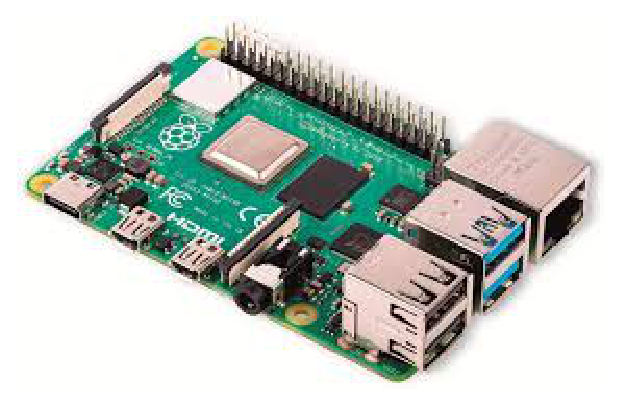
\includegraphics[clip, width=4.5cm]{./fig/chap2/raspi4b.eps}
          \hspace{1.6cm} Raspberry Pi Model 4 B \cite{model4B}
        \end{center}
      \end{minipage}

      % 2
      \begin{minipage}{0.33\hsize}
        \begin{center}
          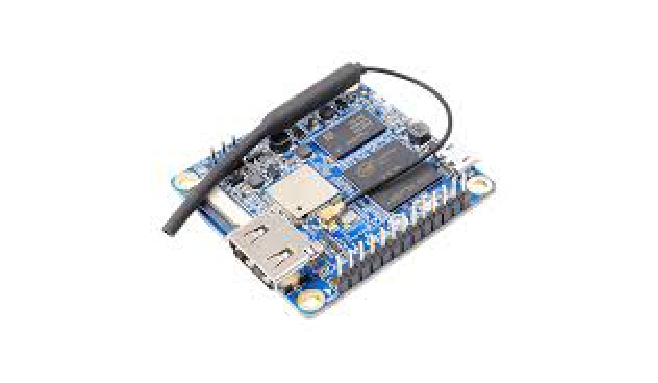
\includegraphics[clip, width=6.0cm]{./fig/chap2/orenge_pi.eps}
          \hspace{1.6cm} Orange Pi Zero Plus2 \cite{orengepi}
        \end{center}
      \end{minipage}

      % 3
      \begin{minipage}{0.33\hsize}
        \begin{center}
          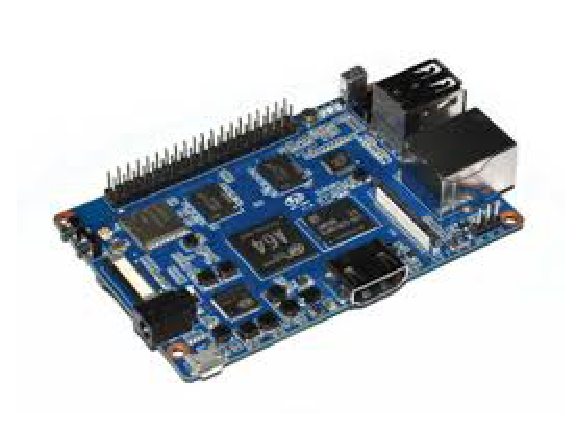
\includegraphics[clip, width=4.5cm]{./fig/chap2/banana_pi.eps}
          \hspace{1.6cm} Banana Pi BPI-M64 \cite{bananapi}
        \end{center}
      \end{minipage}

    \end{tabular}
    \caption{主なSBCの画像}
    \label{fig_2.3}
  \end{center}
\end{figure}



SBCが持つCPUの特徴は,主に低周波数のコアがデュアルコア,クアッドコアなどの形式で複数搭載されている機種が多いことである.
低周波数コアを複数搭載している目的は消費電力を抑えることと価格を低く抑えることであり,こうした省電力や低価格という特徴を維持しつつCPU自体の処理能力を向上させる目的で近年ではコア数の増加が進んでおり,マルチコア方式を採用した機種が多く販売されるようになってきている.
搭載メモリや通信帯域に関しては近年のSBCの性能向上により4.0 GB以上の比較的大きなメモリ容量を持つものも増えており,ギガビットイーサネットに対応したNIC (Network Interface Card) を有するものも多く発売されるようになってきている.
映像出力の機能としてはほとんどの機種でHDMI端子による出力が可能であり,Full HD 解像度での出力が標準的である.
また,各機種のOSには軽量なLinuxベースのOSが広く採用されている.
例えばRaspberry Piに対応したOSであるRaspbian \cite{raspbian}もLinuxをベースとするOSの一種である.



\section{先行研究で提案されたマルチディスプレイシステム}

2.1節で述べたように,ハードウェアを用いたマルチディスプレイの構築ではハードウェア自体の価格によりマルチディスプレイシステムの構築コストが増大する.
また,ミドルウェアを用いてマルチディスプレイシステムを構築する場合でも,ディスプレイと1対1で接続して映像の表示を制御する役割を担うディスプレイノードとして動作する汎用PCが複数台必要になるため同様に構築コストが増大する.
このようなマルチディスプレイシステム構築におけるコスト面の問題に対して,マルチディスプレイシステムの構築費用を低減する目的でディスプレイノードとしてSBCを活用するミドルウェアが開発された.

本節では,先行研究 \cite{Ishida}で提案された,SBCを用いて構築されたマルチディスプレイの特徴について述べる.
まず,マルチディスプレイを構築する各ノードの動作について説明する.
その後フレームの連携表示処理を可能にする仕組みについて概説する.

\subsection*{連携表示処理}

先行研究で構築されたマルチディスプレイシステムは,1台のヘッドノードと,SBCを用いて実装された複数台のディスプレイノードで構成されている.

システムの概要を図\ref{fig_2.4}に示す.

\begin{figure}[H]
  \hspace*{\fill}
  \includegraphics[width=\linewidth]{./fig/chap2/system_4.eps}
  \hspace*{\fill}
  \caption{SBCを用いて構築したシステムの概要図}
  \label{fig_2.4}
 \end{figure}

このマルチディスプレイシステムは,2.1節で述べた2種類の方式のうちフレーム転送方式を採用している.
そのためSBCをディスプレイノードとして用いることとなり,従来のフレーム転送方式をそのまま適用するとSBC上で負荷の高い処理を行う必要がある.
しかし,SBCは市販の汎用PCと比較すると処理速度,描画性能などの面で劣っているため,可能な限りディスプレイノード上での処理負荷を小さく抑えなければならないという制約が存在する.
そのためSBCがディスプレイノードとして十分高速に動作するような設計を目的として,JPEG圧縮や連携表示処理のパイプライン化などが実装されている.

以下では,先行研究において提案されたマルチディスプレイシステムの詳細な動作について述べる.
ヘッドノードでは動画ファイルからフレームを切り出した後,接続ディスプレイノード数に応じてフレームの分割を行う.
分割したフレームはそれぞれJPEG方式で圧縮され,各ディスプレイノードへと送信される.
ヘッドノードから送信された圧縮フレームを受信したディスプレイノードでは,フレームを展開し,その展開が終了した後表示バッファに格納してヘッドノードに表示準備完了メッセージを送信する.
ヘッドノードは全てのディスプレイノードからの表示準備完了メッセージを受け取り次第表示命令を送信し,命令を受け取ったディスプレイノードはディスプレイ上にフレームを表示する.

また,ノード上の各処理はスレッド処理によって行われており,ヘッドノード上では圧縮スレッド,送信スレッド,同期制御スレッドの3種類,ディスプレイノード上では受信スレッド,展開スレッド,表示制御スレッドの3種類のスレッドが動作している.

各スレッドの操作を図\ref{frow_system}, 図\ref{thread_flow}に示す.

圧縮スレッドは表示映像の切り出しと分割,圧縮までを行う.
送信スレッドは,圧縮されたフレームを各ディスプレイノードに送信する.
同期制御スレッドは,表示準備完了メッセージの受信と表示命令の送信を行う.
受信スレッドは,ヘッドノードから圧縮フレームを受信する.
展開スレッドは,圧縮フレームの展開を行う.
表示スレッドは,ヘッドノードからの表示命令を受け取りフレームをディスプレイ上に表示する.

\begin{center}
  \begin{figure}[H]
      \hspace*{\fill}
      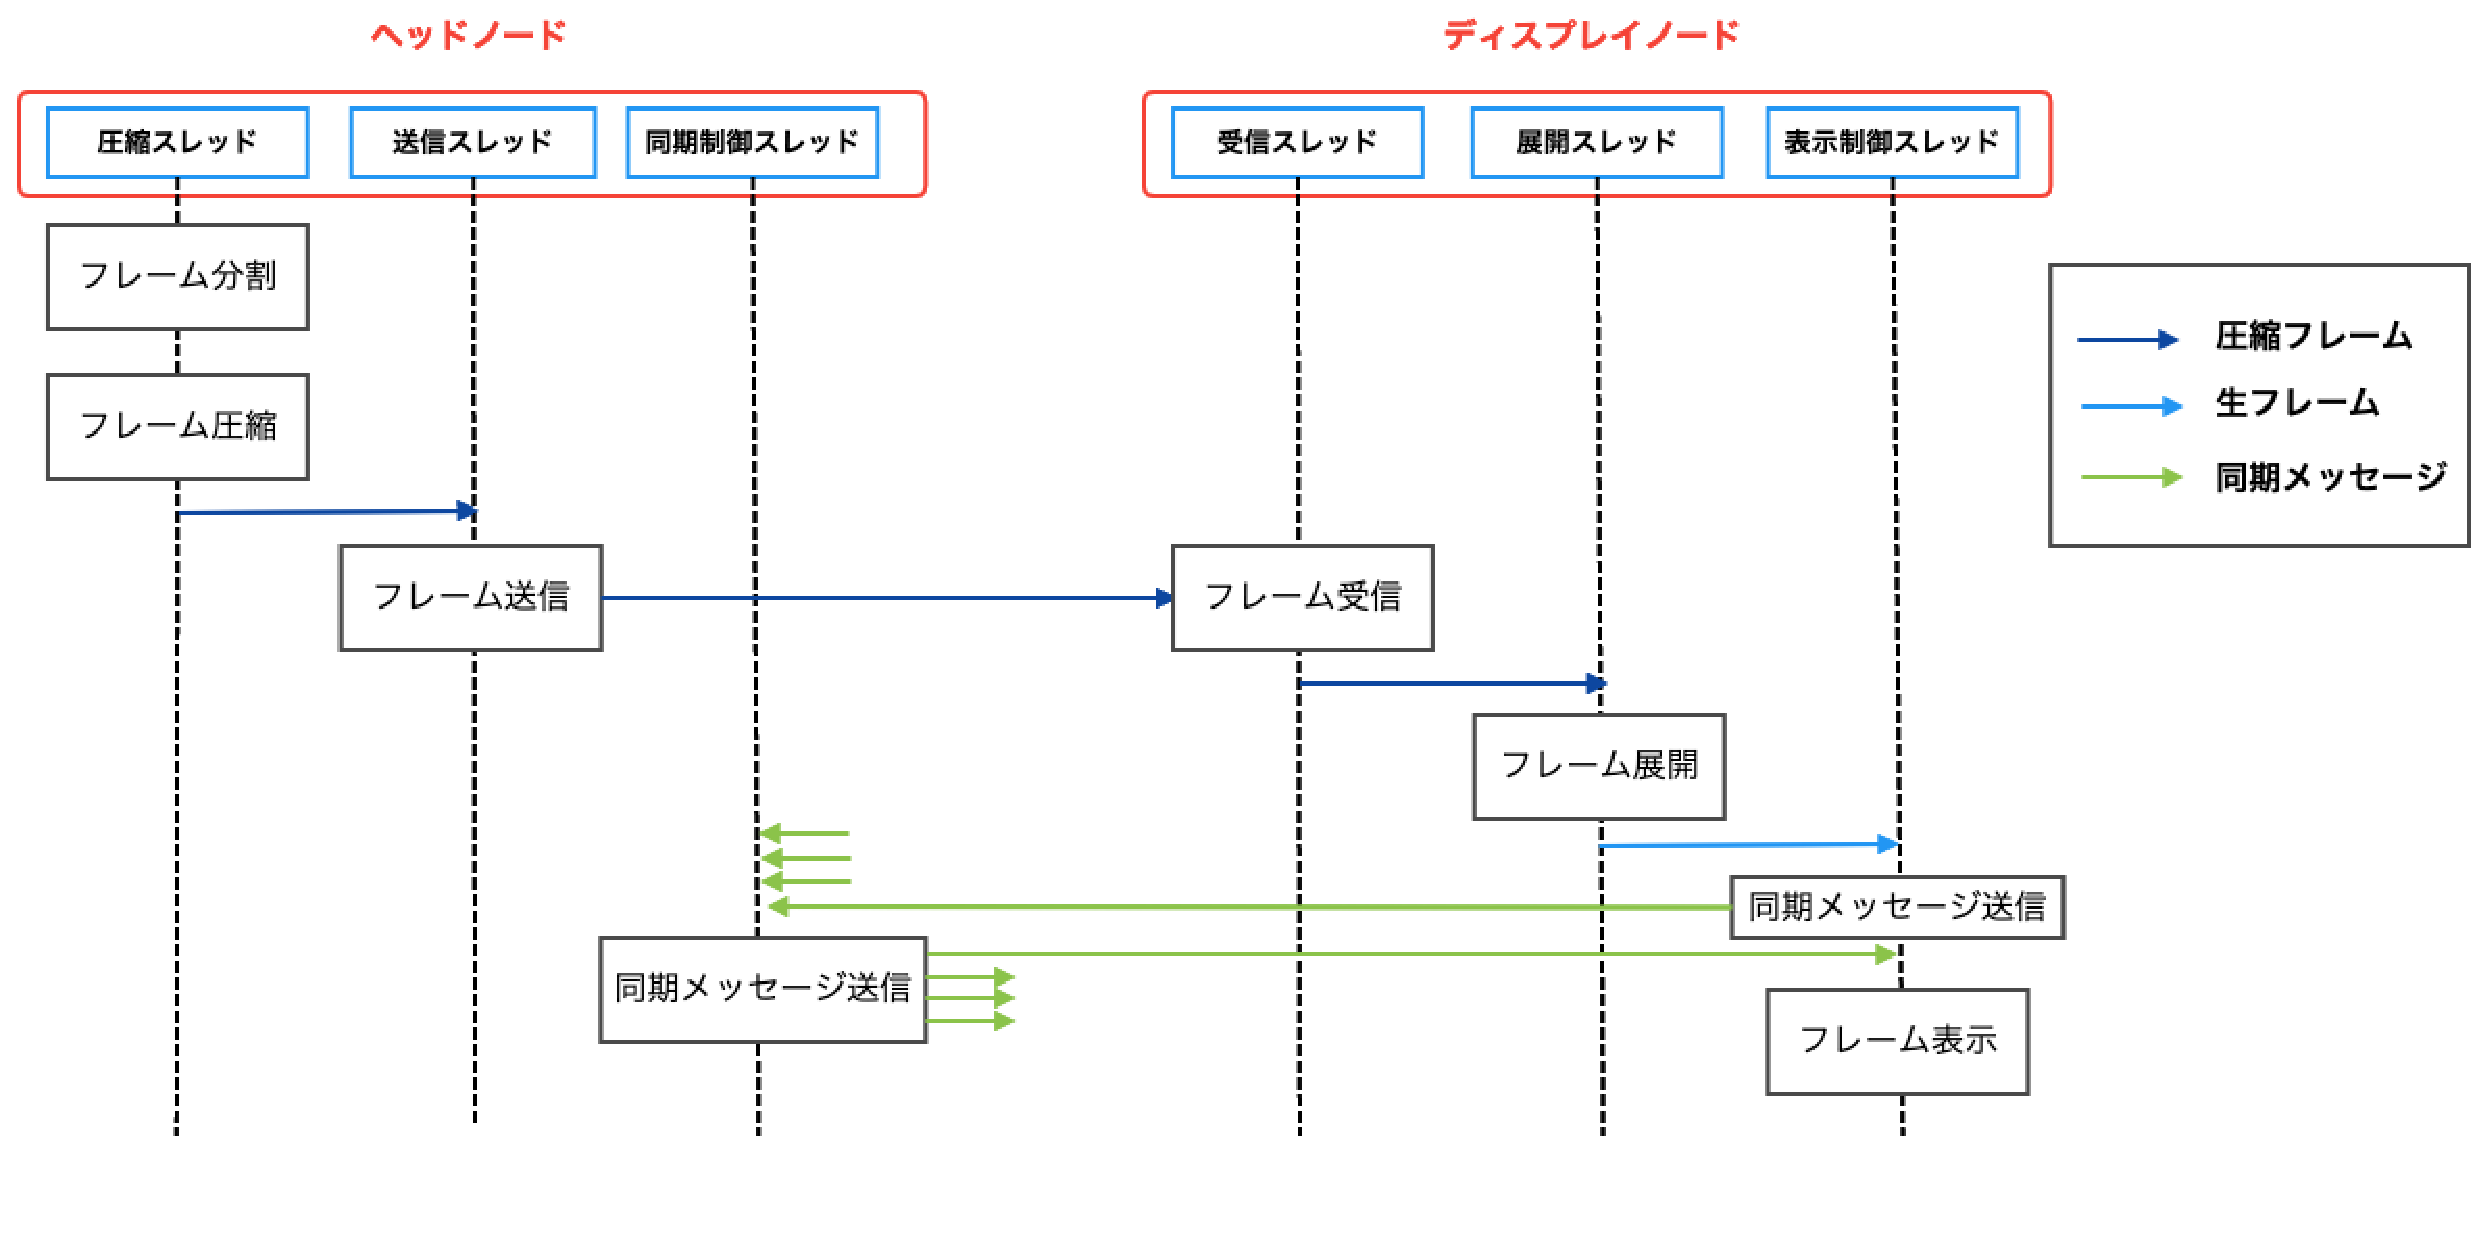
\includegraphics[width=1.1\linewidth]{./fig/chap2/frow_system.eps}
      \hspace*{\fill}
      \caption{各スレッドの動作}
      \label{frow_system}
  \end{figure}
  \end{center}

  \begin{center}
    \begin{figure}[H]
        \hspace*{\fill}
        \includegraphics[width=1.1\linewidth]{./fig/chap2/previous_thread.eps}
        \hspace*{\fill}
        \caption{各スレッドの動作}
        \label{thread_flow}
    \end{figure}
    \end{center}
   

\subsection*{フィードバック処理}

JPEG圧縮処理では,まず入力画像のピクセルごとの画素値をRGB形式からYCbCr形式に変換する.
YCbCrは色彩表現法の一種であり,色を人間の目が認識しやすい輝度成分と人間の目では認識しづらい色差成分とに分けて表現する\cite{YCbCr}.
YCbCr形式に変換された色成分はデータ量を削減するために間引かれることになるが,このときYCbCrサンプル比という間引き方を決定するパラメータを変更することで,JPEG圧縮に要する時間を変更することができる~\cite{jpeg2}.
また,量子化を行う際の品質係数と呼ばれるパラメータを変更することによってもJPEG圧縮に要する時間を短縮することができる.
先行研究のマルチディスプレイシステムでは,ディスプレイノードで動画再生時のフレームレートを計算し,目標フレームレートとの差に応じてこれらのパラメータを変更することでフレームレートを目標値に近づけるフィードバック処理を実装している.

\section{問題点と技術的課題}

本節では,前節で述べた先行研究におけるマルチディスプレイシステムの問題点と,それを解決するための技術的課題について述べる.
まず,先行研究のマルチディスプレイシステムにおける具体的な問題について説明する.
その後,問題点解決に向けた手法の考察と利点,欠点について述べ,比較を行う.

\section*{先行研究で提案されたマルチディスプレイシステムの問題点}

先行研究で構築されたマルチディスプレイには,高解像度な動画や高フレームレートな動画を表示しようとするとパフォーマンスが低下するという問題点がある.
この問題の原因となっているのが,ヘッドノードでのフレーム処理である.
前述したように,ヘッドノード内では動画フレームに対して分割,圧縮,送信の3つの処理が行われている.
高解像度な動画では1フレームあたりのデータ量が大きくなるためフレームの圧縮に時間がかかり,マルチディスプレイのパフォーマンスが低下する.
また,高フレームレートな動画ではフレーム処理に要する時間が動画における1フレームの表示時間を上回るため,動画本来のフレームレートを維持したまま動画を再生することが困難になる.

また,大規模なマルチディスプレイを構築した場合におけるマルチディスプレイのパフォーマンス低下も問題点として挙げられる.
先行研究で構築されたMDの中では圧縮スレッド,送信スレッド,同期制御スレッドがそれぞれ単一のスレッドとして動作している.
マルチディスプレイを構成するディスプレイの数が増加した場合にはそれに伴ってフレーム圧縮処理の回数も増加し,圧縮スレッドでのフレーム処理負荷も同様に増加することとなる.
しかし,ヘッドノード内で動作する圧縮スレッドは1つであるため,処理負荷の増加に伴って処理に要する時間も増加することとなり,動画再生時のフレームレート低下を引き起こす.
実際,4面構成の場合では30fpsの動画をマルチディスプレイ上に20〜22fps程度で再生することが可能だが,ディスプレイを9面構成にしたマルチディスプレイでは8〜10fps程度に低下することが確認できる(図\ref{framerate_49}).

\begin{figure}[H]
  \hspace*{\fill}
  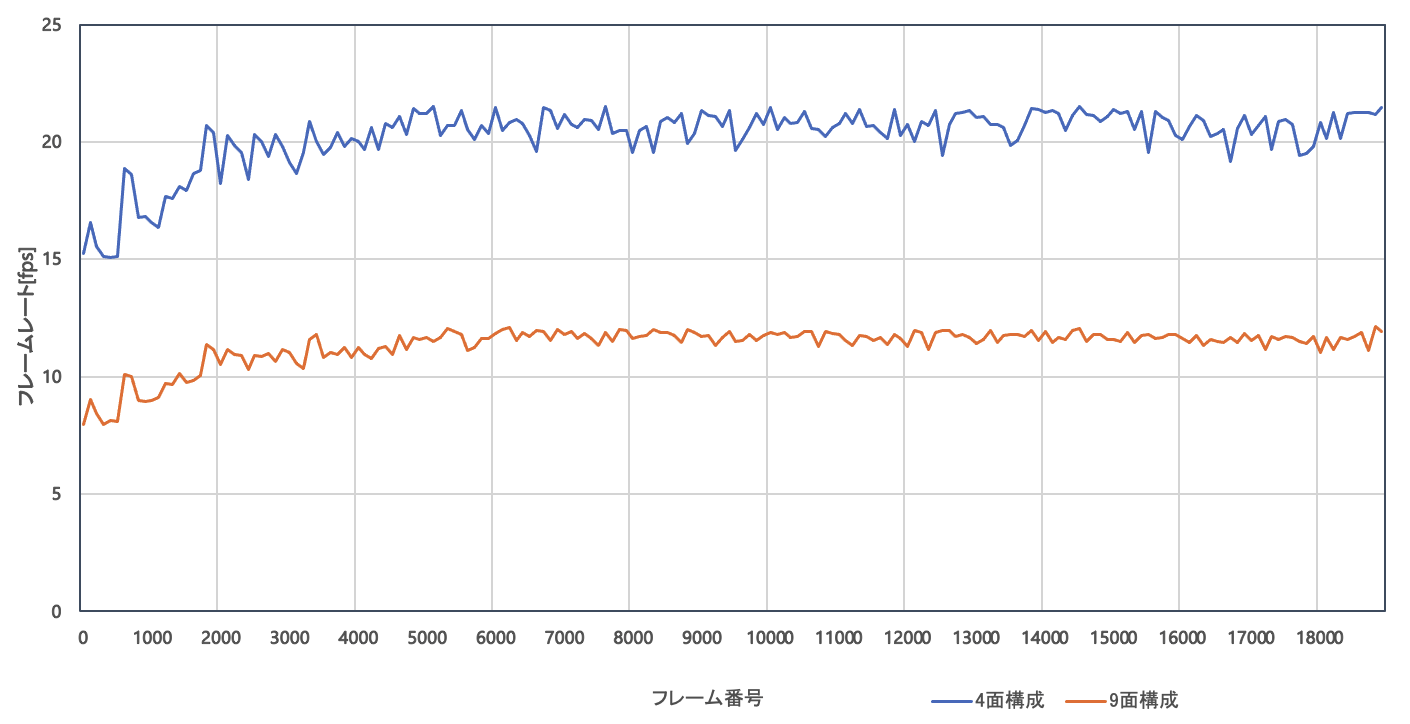
\includegraphics[width=\linewidth]{./fig/chap2/49.eps}
  \hspace*{\fill}
  \caption{画面構成変更時のフレームレート比較}
  \label{framerate_49}
 \end{figure}


 \section*{ヘッドノードの処理負荷軽減を行った関連研究}
 
ヘッドノード上でのフレーム処理負荷が増加しフレームレートが低下するという問題に対して有効な手法として,ヘッドノード上でのフレーム処理を並列化することにより処理負荷を軽減し,フレーム処理に要する時間の短縮を試みることが考えられる.
この手法を用いた関連研究として,自身の卒業研究がある.

\subsection*{実装の概要}

関連研究では,ヘッドノード上での処理を分散並列化する目的で処理のノード分散を行っている.
ノード分散では新たにノードとしてCPUを追加実装することによって物理的にCPUを増加させ,高負荷なフレーム処理を複数のCPUで分担して実行する.
また,ヘッドノードの性能に依存することが少なくなるため,ヘッドノードとしてCPUコア数が少ないような比較的低価格なPCを用いた場合にも大きく性能を落とさずに動作することが期待できる.

関連研究では,ヘッドノードの処理を複数のノードに分散するためにヘッドノードとディスプレイノードとの間に新たにSBCを用いて中継ノードを実装した.
また,連携表示処理の並列化を行うため中継ノード上での処理を受信スレッド,画像処理スレッド,送信スレッドという3種類のスレッドで分担して行うようマルチスレッド化している.

各スレッドの動作を図\ref{middle_flow}に示す.

\subsection*{中継ノードの動作}
受信スレッドはヘッドノードから送信される一次分割済み非圧縮画像フレームを受信し,受信バッファへの格納を行う.
分割・圧縮スレッドは受信バッファに格納された非圧縮フレームを取り出し,接続されているディスプレイノードの数に応じてフレームの二次分割処理を行う.
その後,それぞれの分割済フレームに対してJPEG圧縮処理を行い,送信バッファへと格納する.
送信スレッドは,送信バッファに格納されたJPEG圧縮済フレームを各接続ディスプレイノードへと送信する処理を行う.
以上の3種類のスレッドによって,中継ノードはヘッドノードとディスプレイノードとの間で連携表示処理を実現する.

\begin{figure}[H]
  \hspace*{\fill}
  \includegraphics[width=\linewidth]{./fig/chap2/frow_middle.eps}
  \hspace*{\fill}
  \caption{各スレッドの動作}
  \label{middle_flow}
\end{figure}

\subsection*{ヘッドノードの動作}
中継ノードを実装したマルチディスプレイシステムでは,ヘッドノードはまず動画ファイルからのフレーム切り出しを行い,接続された中継ノード数に応じた分割処理を行う.
分割された画像フレームは送信スレッドへ渡され,各フレームに対してフレーム番号が付与される.
そして,フレーム番号の付与が終了したフレームは圧縮処理を行わずに中継ノードへと送信される.

\subsection*{ディスプレイノードの動作}
ディスプレイノードは中継ノードから送信された圧縮フレームを受信し,受信バッファに格納する.
その後,展開スレッドが圧縮フレームを展開する.
展開処理が終了したフレームは表示バッファに格納され,表示制御スレッドがこれを認識してヘッドノードへ表示準備が完了した旨の同期メッセージを送信する.
そして,ヘッドノードからの表示命令を受信し,表示制御スレッドが表示フレームの切り替えを行うことにより順次フレームがディスプレイ上に表示される.
この一連の動作を繰り返すことにより,マルチディスプレイシステムとしての連携表示処理が可能となる.

図\ref{middle_mdflow}に提案手法を用いて構成した4面構成のマルチディスプレイシステム全体の論理構成図と動作フロー図を示す.


\begin{figure}[H]
  \hspace*{\fill}
  \includegraphics[width=\linewidth]{./fig/chap2/system_figure.eps}
  \hspace*{\fill}
  \caption{関連研究で提案された手法を用いたMDの動作フロー}
  \label{middle_mdflow}
 \end{figure}

 \subsection*{関連研究の問題点と将来課題}
関連研究の評価では,中継ノードを実装した効果を検証するため,先行研究と提案手法において9面
構成のMDを構築して4K解像度の動画再生時におけるCPUコア使用率を計測した.
先行研究ではHNのCPUコア使用率が100\%近くに達していたのに対して,関連研究での提案手法では20\%以下に抑えられていた.
また,中継ノードのCPUコア使用率もも70\%程度となり,分散並列処理によるCPUコア時間のボトルネックは解消された.
しかし,フレームレートなどシステムのパフォーマンスの面では元々のマルチディスプレイシステムと比較して性能が低下した (表\ref{framerate_comp}).

 \begin{table}[H]
  \centering
  \caption{中継ノード実装によるフレームレートの比較}\label{tab1}
  \scalebox{1.2}{
  \begin{tabular}{cccc}
  \hline
  手法 & 平均 & 最大 & 最小\\
  \hline
  中継ノード実装システム & 1.95 & 2.25 & 1.85\\
  中継ノード非実装システム & 9.44 & 10.42 & 7.35\\
  \hline
  \end{tabular}
  \label{framerate_comp}
  }
  \end{table}

 原因として考えられるのは,中継ノードを新たに実装したことで生じたフレームの送受信処理である.
 関連研究で提案されたマルチディスプレイシステムでは中継ノード内で画像フレームの圧縮処理を行うため,画像フレームはまずヘッドノードから中継ノードへと送信され,中継ノードで圧縮処理がなされた後ディスプレイノードへと送信される.
 この2度のフレーム送受信処理によって生じるオーバーヘッドが影響し,システムのパフォーマンスが低下したと考えられる.

 \section{関連研究での技術的課題}
関連研究では,ヘッドノードでのフレーム圧縮処理を分散並列化する目的で複数の中継ノードをヘッドノードとディスプレイノードの間に設置した.
しかし,前節で述べたようにヘッドノードのCPU使用率は低下したものの,マルチディスプレイシステムのパフォーマンス指標として最も重要なフレームレートは大幅に低下していた.
この結果から,ヘッドノードの処理を外部のノードへ分散させる手法はCPUの負荷分散に対しては効果的であるが,マルチディスプレイシステム自体のパフォーマンス向上には貢献できていないと考えられる.
すなわち,関連研究での技術的な課題は,ヘッドノードの処理の分散を外部のノードを用いて行うのではなく,ヘッドノード内のリソースを効率的に活用してフレーム処理の分散化を行うことである.
ヘッドノード内のCPUリソースを活用することで,フレームデータ送受信のオーバーヘッドを生じさせずにフレーム処理の並列化を行う事ができ,フレームレートの向上にも寄与できる可能性が高い.

図\ref{cpuusage}に,関連研究のヘッドノードにおけるCPU使用率の推移を示す.

\begin{figure}[H]
  \hspace*{\fill}
  \includegraphics[width=\linewidth]{./fig/chap2/cpurate_head_proposed.eps}
  \hspace*{\fill}
  \caption{関連研究のヘッドノードにおけるCPU使用率}
  \label{cpuusage}
 \end{figure}

これは中継ノードを実装して構築したマルチディスプレイ上に4K解像度の動画を表示し,映像の表示開始から300秒間のヘッドノードにおける各CPUコアの使用率の推移を計測したものである.
最も使用率が高い瞬間においても使用率は15\%程度にとどまっており,ヘッドノードの計算能力には十分な余裕が存在していることが確認できる.
この計算能力の余裕を活用することでヘッドノード内で完結した処理が可能となり,画像フレームデータ送受信のオーバーヘッドを生じないフレーム処理が可能になると考えられる.

本研究では,SBCを用いて構築したマルチディスプレイに対してボトルネックとなっているフレーム処理部分の改善とMDのパフォーマンス向上を目的として設定し,ヘッドノード内のCPUリソースを活用したフレーム処理機構の実装について取り組む.


